\documentclass[oneside]{tongjithesis}
\usepackage{tongjithesis}

%%%%%%%%%%%%%%%%%%%%%%%%%%%%%%%%%%%
% 若你想要用句点(.)替换句号(。)
% 可以打开下面的注释
%%%%%%%%%%%%%%%%%%%%%%%%%%%%%%%%%%%
% \catcode`\。=\active
% \newcommand{。}{\ifmmode\text{.}\else .\fi}
%%%%%%%%%%%%%%%%%%%%%%%%%%%%%%%%%%%

%%%%%%%%%%%%%%%%%%%%%%%%%%%%%%%%%%%
% 在Windows上使用时:
% 若你想避免将 Python 加入环境变量,可以在此手动指定python环境
% 打开下面的注释,并替换尖括号<>中的路径
% e.g. {<X:/your/path/to/python>/python.exe} -> {C:/software/Anaconda3/envs/latex/python.exe}
%%%%%%%%%%%%%%%%%%%%%%%%%%%%%%%%%%%
% \newcommand{\myPython}{<X:/your/path/to/python>/python.exe}
% \renewcommand{\MintedPygmentize}{\myPython\space -m pygments}
%%%%%%%%%%%%%%%%%%%%%%%%%%%%%%%%%%%

\newcommand{\myPython}{C:/software/Anaconda3/envs/latex/python.exe}
% \newcommand{\myPython}{C:/Users/didik/anaconda3/envs/latex/python.exe}
\renewcommand{\MintedPygmentize}{\myPython\space -m pygments}

\DeclareSIUnit{\Hu}{Hu}

\begin{document}

\school{电子与信息工程学院}
\major{计算机科学与技术}
\student{1950084}{陈泓仰}
\thesistitle{基于评估函数的自动三维区域生长算法}{}
\thesistitleeng{Automated 3D region growing algorithm based on an assessment function}{}
\thesisadvisor{}
\thesisdate{2023}{5}{19}

\MakeCover


\makeatletter
\@ifclasswith{tongjithesis}{twoside}{%
\cleardoublepage
}{%
\clearpage
}
\makeatother

\pagestyle{firststyle}
\MakeAbstract{
    食道疾病在我国民众中的患病率逐年攀升,针对食道疾病的预防和诊断显得尤为关键。食道造影作为一种简便的检测方法,能够直观地展示食道状况,有效探测食道结构的异常。当前针对DR图像的研究较多,但对连续的图序列的研究较少。本课题对人类食道医学造影视频进行分析,我们提出了一种自动调整窗宽窗位的方法,使关注的钡餐区域更为突出,并采用光流法对视频进行逐帧配准。我们采用降噪、轮廓提取、腐蚀膨胀等图像处理方法,获取了视频数据中每一帧图像里的钡餐区域及其本底值。最后,我们设计了一种拓展逐帧处理成果的方法,依据多帧序列生成最终的钡餐区域及相对浓度标定结果。
}{X线钡餐造影,视频处理,图像分割}

\MakeAbstractEng{
    The prevalence of esophageal diseases in our population is increasing year by year. Therefore, prevention and diagnosis of esophageal diseases are particularly critical. As a simple detection method, esophagogram can visualize the condition of the esophagus and effectively detect abnormalities in esophageal structures. Currently, there are many studies on DR images, but few on continuous image sequences. In this project, we analyze the video and images of human esophagogram, we propose a method to automatically adjust the window width and window level to make the barium meal region more prominent, and use the optical flow method to align the video frame by frame. We used image processing methods such as noise reduction, contour extraction, and erosion expansion to obtain the barium meal region and its background value in each frame of the video data. Finally, we designed a method to extend the frame-by-frame processing results to generate the final barium meal region and relative concentration calibration results based on multi-frame sequences.
}{X-ray barium meal, video processing, image segmentation}


\makeatletter
\@ifclasswith{tongjithesis}{twoside}{%
\cleardoublepage
}{%
\clearpage
}
\makeatother

\tableofcontents   %放置目录

\makeatletter
\@ifclasswith{tongjithesis}{twoside}{%
\cleardoublepage
}{%
\clearpage
}
\makeatother

\pagestyle{mainstyle}
\section{绪论}\label{sec:1}

\subsection{研究背景及意义}

随着社会的进步和生活水平的不断提高,人们的生活节奏加快,饮食习惯和生活方式改变,小酌喝酒、暴饮暴食等都可能对食道产生不良影响。加之疾病因素、遗传因素等原因,导致食道疾病在国人中的发病率逐年上升。食道疾病包括食道炎、食道裂孔疝、食道癌等,在现代社会已成为常见病患问题之一,对患者的生活质量和身体健康带来较大影响。因此,针对食道疾病的预防和诊断显得尤为重要。

食道造影作为一种检查手短,能对食道进行直观显示,有效地检测食道结构异常。食道医学造影图像分析的研究对于食道疾病的诊断、评估治疗方案和监测疗效具有重要意义。在进行食道造影操作时,对硫酸钡浓度的关注至关重要,以免过低或过高影响疾病的检出率。针对不同患者的吞咽能力,应该配置适宜黏稠度和浓度的造影剂。然而在实际检查过程中,医生常常依赖主观判断造影剂的黏稠度,缺失客观的参考标准,致使患者在接受检查时可能面临误吸和呛咳等风险。

本课题旨在通过对人类食道医学造影视频与图像的深入分析,准确标识不同浓度钡餐在食道内的分布区域,并运用计算机图形学相关算法,构建流动钡餐在双重视角的封闭几何范围。结合后续课题,这项研究将有助于提高食道疾病的诊断准确性、降低误诊或漏诊率,并能对疾病的评估和治疗方案提供数据支持。此外,借助计算机技术,能够进一步推动食道影像诊断技术的发展,为解析更多健康隐患和降低医疗成本奠定基础,帮助患者对自身食道疾病的认识和预防增加信心。

\subsection{国内外研究现状}

医学影像技术在食道检测方面发挥着重要作用,其中 X 射线便是医疗界常见的初步筛查方法之一。X 射线始于 1859 年,由德国物理学家、诺贝尔物理学奖得主威廉·康拉德·伦琴发现\cite{johansen1996circumstances}。自 X 射线被发现后,其在医学影像诊断技术中的潜在应用便迅速被确认,并广泛应用于全身各组织器官的检查。在 X 线造影检查过程中,人体不同器官与组织的密度与厚度差异导致其在影像上呈现出自然的黑白层次对比效果。如今,利用 CR(计算摄影)系统(核心部件为 IP(成像板))的技术,光信号可转换成电信号,进而以电子数据形式储存。X 射线影像中展现的信息(包括不同明暗/黑白对比的像素)质量与数量取决于被照射对象的因素(例如原子序数、密度、厚度)以及射线本身的诸多因素(例如线质、线量、散射线等)。

在许多情景下,为了使造影图像更加清晰,需要使用对人体无害的造影剂。对于钡、碘等元素,由于其原子系数较大,与 X 射线发生光电效应时会产生特征 X 射线。这些射线能够穿透人体组织,形成灰雾效果的影像,使显示对比度提高,达到理想的检测效果。这种检查方法在临床医学上被称为 X 线钡餐造影检查。钡餐造影,亦即上消化道钡剂造影检查,是让受检者摄取糊状硫酸钡(显影剂)后,在 X 线照射下查看消化道是否存在病变的检测方法。硫酸钡既不溶于水,也不溶于脂质,因此不会被胃肠道黏膜吸收,对人体基本上无毒性。以果仁、小鱼刺为例,一些透 X 线的异物无法直接被显影,这些异物被称为食管阴性异物,需通过钡剂造影方能诊断。较大的异物在吞服钡剂后,在透视下可见钡剂流向异物处受阻,形成分流或偏流绕过异物下行。此外,细小异物也可通过向钡剂中加入棉絮来检测,在透视下观察到钡絮钩挂,即使在吞咽或饮水操作后,钡絮仍不下行,可指示异物所在位置。

\subsubsection{静态图像分析}

本课题首先应对医学视频数据的逐帧画面进行静态分析。尽管目前国内外在数字化X线钡餐造影领域的研究颇为丰富,然而在钡餐范围标定以及浓度方面的探讨却相对不足。据查阅,仅有2021年一项涉及此领域的研究成果。在该成果中,吴越等学者探讨了不同钡餐浓度及增稠剂浓度对患者吞咽舒适度的影响\cite{wu2021}。

有鉴于此,我进一步检索了关于其他医学影像分割或标注方面的研究。国内外关于医学影像的分割与标注领域研究繁盛,包括传统方法及深度学习方法两大发展方向。传统的分割技巧有基于模糊聚类法、基于区域生长法、基于形态学分水岭法、基于可变形模型法、基于异常检测法、基于图谱匹配法等。在众多方法中,分水岭算法与区域生长分割以其精准、迅速、高效的特点而备受青睐。分水岭算法最初由 Digabel 和 Lantuejoul 率先引入图像处理领域\cite{wang2009watershed},而由柴\cite{chai2007watershed}等提出的改进版分水岭算法,尽管在抗噪声方面有了显著提升,但仍不免出现过分割的现象等。基于深度学习的分割方法主要使用全卷积神经网络(FCN)\cite{2015Fully},结合U-Net\cite{Ronneberger2015}或Dense-Net\cite{huang2017densely}网络进行优化。

由于钡餐浓度随时间变化大,且在不同器官中的形态变化大,传统的分割方法均无法取得较好的效果。而基于深度学习的分割方法主要面临缺乏公开数据集的问题。同时,食道X线钡餐造影图像涉及多方位和多器官,难以将网络进行迁移学习、训练和应用。

\subsubsection{动态图像分析}

想要更加准确地描绘钡餐分布区域以及其浓度变化,还需结合连续时间片所带来的流动参数信息及运动形态变化信息。目前,国内外关于二维医学视频的连续标注研究较少。2020年,刘强等人研究了冠脉造影图序列的生理运动补偿减影,通过分解生理运动信号,在不依靠心电门控的前提下完成帧间配准\cite{liu2020}。在其它领域,当前针对视频目标跟踪的研究主要聚焦于小样本学习或弱数据标注,无监督学习或缺陷数据集,多目标或特定目标跟踪,以及提升速度和稳定性等方面。

本课题所涉及的数据样本规模较小,目标形态差异较大,且对标注精度要求高。根据以上分析,目前相关领域尚缺乏成熟研究成果与稳定的算法模型。本课题的研究内容具有创新性,前置研究较少,面临一定挑战。

\subsection{论文的结构安排}

本文的研究重点是对输入的医学影像数据进行逐帧标注,准确描绘钡餐分布区域以及其浓度变化。为更出色地完成本课题研究,我们采用多种医学及图形学算法,包括:窗口调节、图像配准、图像去噪,以及轮廓的提取、计算及形变等技术。最后,我们提出了一种基于图像处理的算法,充分利用时域信息,使用前驱帧处理结果扩展当前帧处理结果。

本课题所采用的各组数据均存储于独立的DIC格式文件中,数据类型为DICOM医学影像。DICOM(数字成像和通信标准)是一种在放射学、心血管以及其他医学领域广泛应用的医学影像格式,其文件中包含影像以及患者、设备和诊断信息等元数据。在本课题研究中,每组数据对应一次独立的X线检查,以连续时间片的形式记录了钡餐在受试者体内的二维图像。图像为受试者的侧位头部及颈部。在每次检查过程中,研究人员会通过针筒将定量钡餐注入受试者口腔。钡餐可能出现于受试者的口喉、咽部或食道;钡餐可能在口腔静止,被吞咽或被吐出。

本文结构如下:

第一章:绪论

本章首先阐述了本文的研究背景和意义。本课题对X线检查生成的医学视频数据进行标注,描绘钡餐分布区域及浓度。本章综合概括了与本课题相关的算法在国内外的研究现况。最后,以论文的组织结构为线索,对本文的主要内容进行阐述。

第二章:医学视频预处理与优化

本章将对待处理的视频数据进行预处理。首先运用自动窗宽窗位算法,凸显出我们所关注的钡餐区域;接着从数据中提取运动形态变化信息,并采用光流法对视频进行逐帧配准,为后续逐帧图像分析处理奠定基础。

第三章:逐帧图像处理研究

本章应用多种图像处理算法,提取视频数据中每一帧图像里的钡餐区域及其本底值。操作流程如下:对相邻帧图像求差值,得到待处理图像;对图像进行去噪处理;使用算法获取图像轮廓及每个轮廓所包围的像素数;循环运用腐蚀和膨胀算法筛选并剔除小轮廓以实现进一步去噪;对上述步骤得到的钡餐区域进行本底值标注,生成最终蒙版。

第四章:基于多帧序列生成标定结果

本章中,我们提出一种拓展逐帧操作成果的算法。针对每一帧图像,以上述获得的蒙版作为基础,借助前驱帧所得蒙版进行扩张操作;在此过程中,不断维护各蒙版的有效性,以提高处理速度。最终,我们得到每一帧中的钡餐区域及相对浓度标定。

第五章:实验结果分析

本章首先将原始数据、蒙版、最终成果同时展示,观察并分析区域标定的准确性。由于原始采集仪器数据及环境数据暂缺,无法确定钡餐的绝对浓度,因此采用相对浓度,并以R通道值形式叠加于原始数据进行展示,以便观察和分析浓度标定的准确性。
\clearpage
\section{医学视频数据预处理与优化}\label{sec:2}

对X线检查得到的DR图像进行预处理是计算机辅助诊断中的重要课题。为衡量生物器官对X射线的吸收率,Hounsfield\cite{peeters1979nobel}定义了描述辐射密度的标准量化单位。CT值的单位被命名为亨氏单位(Hounsfield Unit,简称Hu),以纪念Hounsfield为CT成像所作出的卓越贡献。CT值的计算公式如下:
\begin{equation}
    CT值 = \frac{\mu_m - \mu_w}{\mu_w} \times \alpha
\end{equation}
其中 $\alpha$ 为分度因子。当值取1000时,CT值的单位即为亨氏单位。$\mu_m$ 表示X射线穿透生物组织的衰减系数,而 $\mu_w$ 则代表标准水的衰减系数。亨氏单位将水的衰减系数作为标准,人体各种组织具备不同的衰减系数。在医学图像上,人体组织的 CT值范围一共有2000个单位。在这一数值之中,水的CT值位列中心点,数值为 \SI{0}{\Hu};空气的CT值最低,为 \SI{-1000}{\Hu};骨骼组织的CT值则最高,可达 \SI{1000}{\Hu}。CT值所涵盖的2000个单位远超过了灰度图像所能展现的范围,人眼无法直观分析原始的DR图像。针对某一特定组织,调窗技术可以提供更佳的可视效果,有助于更准确地观察病变区域与标志物范围。人们一般通过调整窗口中心和窗口宽度来完成从 CT 值到显示值的线性转换。窗口宽度指定组织的 CT 值范围,窗口中心指定组织 CT 值范围的中心。调窗技术只是令显示效果让人眼接受,并未对图像的原始信息进行更改。调窗技术对于计算机辅助诊断系统非常重要,为每类图像校准生成一致的对比度和特定的CT中心值。

\subsection{自动窗宽窗位算法}\label{sec:2_1}

本课题所分析的医学视频为受试者的侧位头部及颈部的DR图像。鉴于数据获取过程中,受试者未紧贴采集设备,且在吞咽钡餐时头部运动幅度显著,导致各组数据的累计灰度分布差异较大。因此,有必要对每组数据进行单独的窗宽窗位校正。
\begin{figure}[!htp]
    \centering
    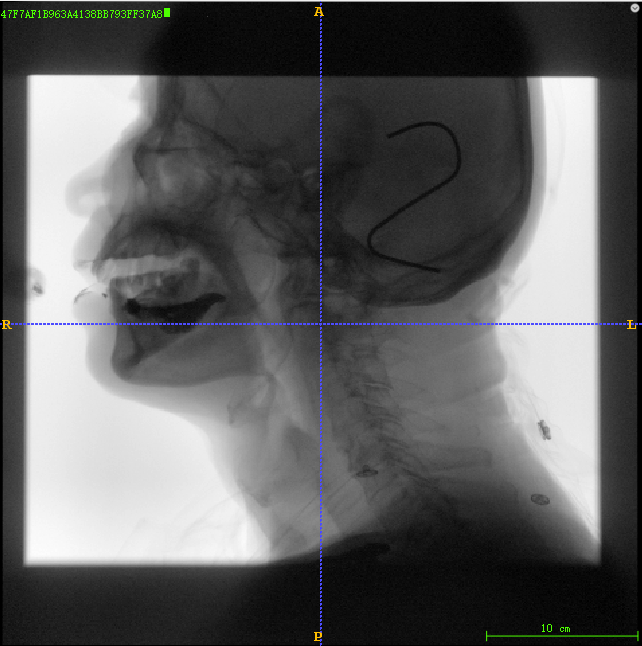
\includegraphics[width=0.4\textwidth]{figures/2_1_1.png}
    %\hspace{1cm}
    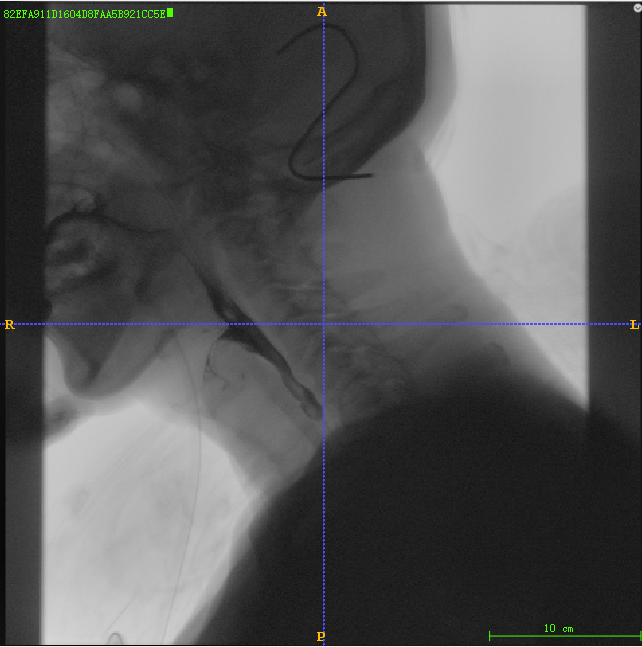
\includegraphics[width=0.4\textwidth]{figures/2_1_2.png}
    \caption{灰度分布差异较大的两组数据的帧截图}
    \label{fig:2_1_原始图像}
\end{figure}

\subsubsection{算法流程}

由于本实验所关注的对象(造影剂)并非人体器官或已被研究的细胞,且在时域中变化较为剧烈,没有已知公认推荐的窗位和窗宽。而人工对每组数据进行矫正耗时较大,且缺乏客观统一的评判标准。因此,本研究采用了基于累积分布函数的自动窗宽窗位算法。基于累积分布图,我们有以下两个普遍假设:
\begin{itemize}
    \item 分布函数的斜率变化反映了整幅图灰度值变化的快慢情况。
    \item 分布函数的斜率越大说明整幅图像的灰度分布越压缩,反之,说明灰度分布宽度越大。
\end{itemize}

最终,本研究采用以下步骤获取窗宽和窗位:
\begin{enumerate}
    \item 从视频中划分出我们感兴趣的区域(喉口和咽部)。在本研究中,该步骤被简化为将视频按固定坐标的矩形裁剪。
    \item 从帧序列中等间隔地提取K张的帧图像。在本研究中,K固定为10。
    \item 对提取出的每张帧图像以 $\frac{1}{K}$ 的权重叠加,得到平均图像。
    \item 对平均图像求取累计分布序列 $S(x)$。即:图像中像素值小于等于 $x$ 的像素总数占图像总像素数的占比为 $S(x)$。
    \item 设定一组阈值区间 $[t_{min}, t_{max}]$。对于所有使得 $S(x)$ 落入阈值区间的 $x$,记录其坐标 $(x, S(x))$ 所形成的集合。在本研究中,$t_{min}$ 固定为0.05,$t_{max}$ 固定为0.95。
    \item 对于上述坐标集合,使用最小二乘法求得拟合直线 $y=kx+b$。
    \item 求得窗位为 $\frac{1-2b}{k}$,窗宽为 $\frac{1}{k}$。
\end{enumerate}

\subsubsection{结果}

\cref{fig:2_1_对比} 展示了两组基于上述自动窗宽窗位算法处理前后的对照数据。这两组数据源自不同的受试者,且钡餐位于受试者体内不同位置。可以看出,本研究所使用的算法具有良好的适应性和稳定性。

\begin{figure}[!htp]
    \centering
    \begin{subfigure}{\textwidth}
        \centering
        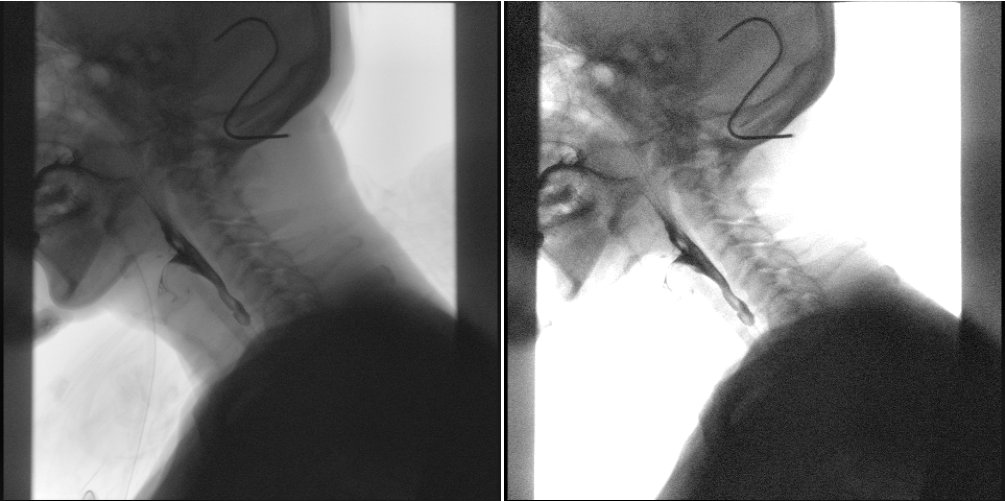
\includegraphics[width=\textwidth]{figures/2_2_1.png}
        \caption{受试者A}
    \end{subfigure}
    
    \begin{subfigure}{\textwidth}
        \centering
        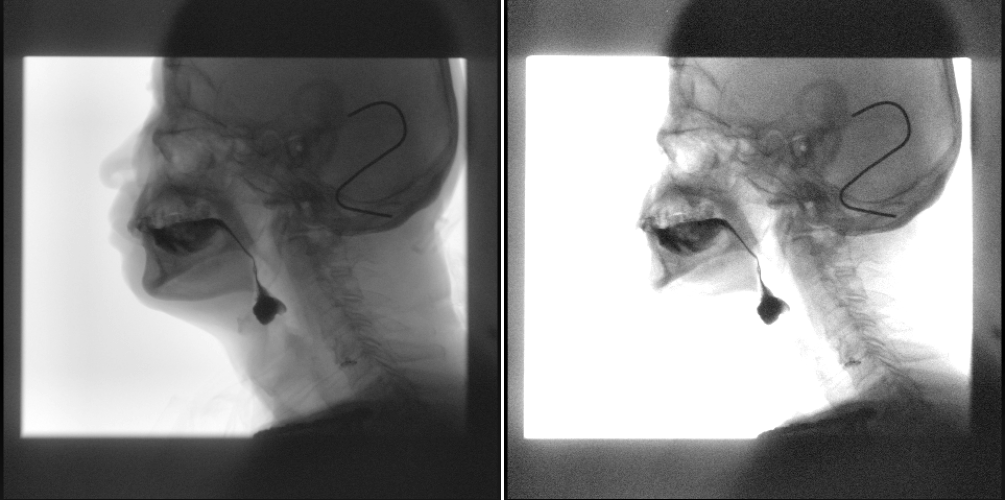
\includegraphics[width=\textwidth]{figures/2_2_2.png}
        \caption{受试者B}
    \end{subfigure}
    \caption{自动窗口算法应用前后对比}
    \label{fig:2_1_对比}
\end{figure}

\subsection{使用光流法配准}\label{sec:2_2}

在本研究的后续章节中,相邻帧图像的差值被用作求钡餐轮廓区域的重要基准。因此,我们需要先对每一帧图像进行配准。

医学图像配准旨在为一幅医学图像寻找一种或多种空间变换,以使其与另一幅医学图像的对应点在空间位置和解剖结构上达到完全吻合\cite{shi2017}。医学图像配准一直以来都是医学图像分析领域的研究热门话题。在众多方法中,基于光流的配准技术成为一种重要的形变配准方式\cite{ji2017based}。

光流概念最早源于计算机视觉领域,其模型可用于表现物体在观测成像平面上像素运动的瞬时速度。图像中每个像素点的运动速度与运动方向所构成的速度场,便被称为光流场。对图像应用光流法,需保证亮同一目标在不同帧间运动时,其亮度不会发生改变。在本课题中,我们主要使用了 Bouguet 和 Jean-Yves 提出的基于金字塔分层的LK光流法\cite{bouguet2001pyramidal}。传统的LK光流法应用在运动速度较快(即相邻帧之间对象的位移较大)的物体上时误差较大。而金字塔LK光流算法利用图像金字塔的多尺度特性,对不同尺度下的图像进行光流估计,从而提高光流估计的准确性和稳定性。

\subsubsection{算法流程}

假设 $u$ 是图像 $I$ 中的一个点,我们要在图像 $J$ 中找到它对应的点 $v$,及对应的变换矩阵 $A$。算法简要流程如下:
\begin{itemize}
    \item 建立 $I$ 和 $J$ 的图像金字塔 \; $\{I^L\}_{L=0,\cdots,L_m} \text{ and } \{J^L\}_{L=0,\cdots,L_m}$
    \item 初始化金字塔上的位移估计为0 \; $\textbf{g}^{L_m}=[g_{x}^{L_m} \; g_{x}^{L_m}]^T=[0 \; 0]^T$
    \item 对 $L_m$ 到 $L_0$ 中的每一个 $L$:
    \subitem 找到 $u$ 在图像 $I^L$ 中的位置 \; $\textbf{u}^L=[p_x \; p_y]^T=\frac{\textbf{u}}{2^L}$
    \subitem 计算 $I^L$ 对 $x$ 的导数 \; $I_x(x,y)=\frac{I^L(x+1,y)-I^L(x-1,y)}{2}$
    \subitem 计算 $I^L$ 对 $y$ 的导数 \; $I_y(x,y)=\frac{I^L(x,y+1)-I^L(x,y-1)}{2}$
    \subitem 计算空间导数矩阵 \; $G=\sum_{x=p_x-\omega_x}^{p_x+\omega_x} \sum_{y=p_y-\omega_y}^{p_y+\omega_y} \begin{bmatrix} I_x^2(x,y) & I_x(x,y)I_y(x,y) \\ I_x(x,y)I_y(x,y) & I_y^2(x,y) \end{bmatrix} $
    \subitem 初始化L-K迭代。对 1 到 $K$ 中的每一个 $k$:
    \subsubitem 图像相减 \; $\delta I_k(x,y)=I^L(x,y)-J^L(x+g_x^L+\nu_x^{k-1},y+g_y^L+\nu_y^{k-1})$
    \subsubitem 计算图像误匹配向量 \; $\overline{b}_k=\sum_{x=p_x-\omega_x}^{p_x+\omega_x} \sum_{y=p_y-\omega_y}^{p_y+\omega_y} \begin{bmatrix} \delta I_k(x,y)I_x(x,y) \\ \delta I_k(x,y)I_y(x,y) \end{bmatrix} $
    \subsubitem 计算光流 \; $\overline{\eta}^k=G^{-1}\overline{b}_k$
    \subsubitem 累加迭代量 \; $\overline{\nu}^k = \overline{\nu}^{k-1} + \overline{\eta}^k$
    \subsubitem 若 $||\overline{\eta}^k||$ 小于设定阈值,打断迭代
    
    \subitem 得到第 $L$ 层的光流估计 \; $\textbf{d}^L = \overline{\nu}^K$
    \subitem 计算出 $L-1$ 层的初步估计 \; $\textbf{g}^{L-1}=[g_x^{L-1} \; g_y^{L-1}]^T=2(\textbf{g}^L+\textbf{d}^L)$
    \item 得到最终的光流估计 \; $\textbf{d}=\textbf{g}^0+\textbf{d}^0$
    \item 定位图像J中的位置 \; $\textbf{v}=\textbf{u}+\textbf{d}$
\end{itemize}

\subsubsection{结果}

\cref{fig:2_2_对比} 展示了一组基于上述光流法处理前后的对照数据。
\clearpage
\begin{figure}[!htp]
    \centering
    \begin{subfigure}{\textwidth}
        \centering
        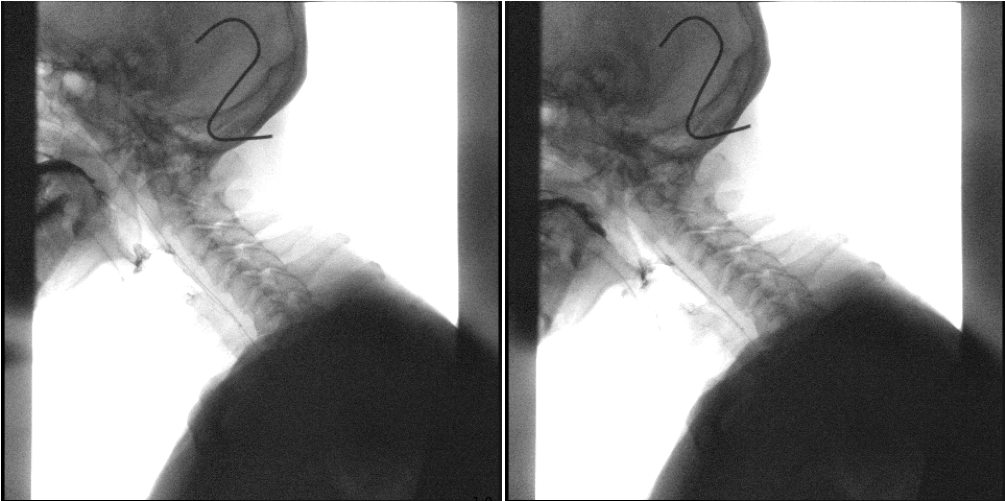
\includegraphics[width=\textwidth]{figures/2_3_1.png}
        \caption{一组数据中的两帧原始图像}
    \end{subfigure}
    
    \begin{subfigure}{\textwidth}
        \centering
        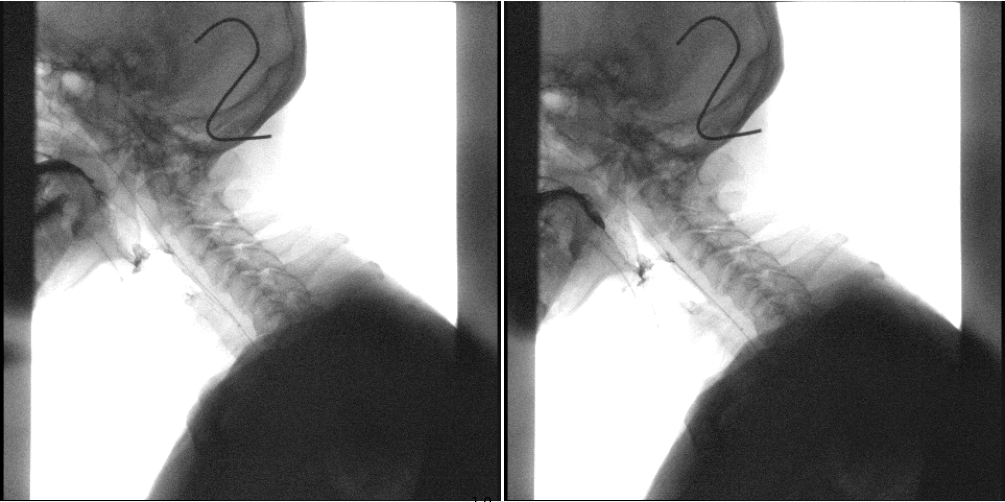
\includegraphics[width=\textwidth]{figures/2_3_2.png}
        \caption{经光流法配准后的两帧图像}
    \end{subfigure}
    \caption{光流法应用前后对比}
    \label{fig:2_2_对比}
\end{figure}

可以看出,该算法抵消了部分受试者的头部运动,为后续逐帧图像分析处理提供正向作用。

\subsection{本章小结}

本章将对待处理的视频数据进行预处理。首先运用自动窗宽窗位算法,凸显出我们所关注的感兴趣区域;接着从数据中提取运动形态变化信息,并采用光流法对图像进行配准,为后续逐帧图像分析处理奠定基础。
\clearpage
\section{评估函数}\label{sec:assessment_function}

\subsection{原理}

$f_{a}(\sigma_{max})$ 的目的是评估区域生长序列中每个元素的分割质量,以检测区域生长过程中的最佳同质性阈值 $\sigma_{opt}$。如果能过程开始时确定最佳阈值 $\sigma_{opt}$,那评估函数将没有作用。但事实并非如此。在过程开始时,由于我们只拥有较为稀疏的目标区域的信息,这种十分困难;在我们的方法中,$\sigma_{opt}$ 由来自分割区域的信息确定。在本文中,分割评估是通过两种方法进行的:按边界或按区域。在第一种情况下,最佳分割对应于边界呈现最强边缘的区域,在第二种情况下,对应于原始图像中最同质的区域。

\subsection{基于边界的方法}

在下文中,边界 $B_{R(\sigma_{max})}$ 一词将用于数学形态学定义的点集,即 $R(\sigma_{max}) \ominus E$,其中 $E = R(\sigma_{max}) \ominus N$,即 $R(\sigma_{max})$ 被 $N$ 二进制侵蚀得到的网状点集,如 \cref{fig:过渡对} 所示,位于边界两侧的两个相邻像素将被称为过渡对(transition couple)。

\begin{figure}[htbp]
    \centering
    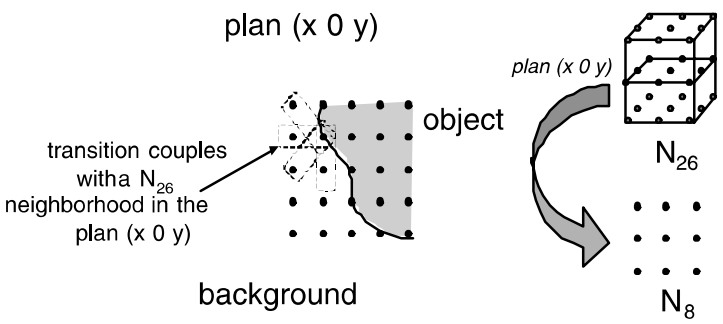
\includegraphics[width=0.6\textwidth]{figures/过渡对.png}
    \caption{过渡对}
    \label{fig:过渡对}
\end{figure}

Kohler(1981)\cite{kohler1981segmentation}提出了一种基于以下启发式的自动阈值方法:对比度越高的边界,越有可能对应于图像中真正的不连续(注意,这种启发式的方法在强对比的纹理图像背景下并不适用)。因此,最佳阈值取决于与该阈值相关的边界中最强的对比度。在我们的应用中,我们概括了Kohler的方法,并提出了 $f_{a}(\sigma_{max})$ 的三个定义,以评估分割后区域边界的质量。

$w_1(\sigma_{max})$ 基于对数图像处理(LIP)对比。Jourlin和Pinoli(1989)\cite{jourlin1989contrast}引入了一个新的数学模型,称为对数图像处理(LIP)模型,特别适合于对数图像,如X射线图像。在这种情况下,他们将两个像素之间的LIP对比度定义如下:
\begin{equation}
    c_f(x,y)=\frac{|f(x)-f(y)|}{1-\frac{\text{min}(f(x)-f(y))}{M}}
\end{equation}
其中 $f$ 是灰阶函数,$M$ 是使得 $2^n$ 严格高于灰阶范围的最低值(例如,如果像素以8比特编码,$M=256$)。

我们定义 $w_1(\sigma_{max})$ 为 $B_{R(\sigma_{max})}$ 的所有过渡对(见\cref{fig:过渡对})的LIP对比之和,以过渡对总数 $N_{tc}$ 标准化:
\begin{equation}
    w_1(\sigma_{\text{max}})=\frac{\sum_{x \in B_{R(\sigma_{\text{max}})}} \sum_{y \in N_x \atop y \notin R(\sigma_{\text{max}})} c_f(x,y) } {N_{tc}}
\end{equation}

$w_2(\sigma_{max})$ 基于标准差。对于 $B_{R(\sigma_{max})}$ 的每个像素 $x$ ,计算x和其不属于分割区域 $R(\sigma_{max})$ 的相邻像素(见\cref{fig:邻域})的标准差,表示为ξ(x)。设 $n$ 为邻居的数量。

我们将 $w_2(\sigma_{max})$ 定义为所有 $\xi (x)$ 的总和,被 $Card\{B_{R(\sigma_{max})}\}$(即:属于 $B_{R(\sigma_{max})}$ 的像素总数)标准化:
\begin{equation}
    \begin{aligned}
    & w_2(\sigma_{\text{max}})=\frac{\sum_{x \in B_{R(\sigma_{\text{max}})}}}{\text{Card}\{B_R(\sigma_{\text{max}})\}}, \\
    & \text{with} \, \xi(x)=\sqrt{\frac{\sum_{y \in N_x \atop y \notin R(\sigma_{\text{max}})}(f(y)-m)^2}{n}} \, \text{where} \, m=\frac{f(x)+\sum_{y \in N_x \atop y \notin R(\sigma_{\text{max}})}f(y)}{n+1} 
    \end{aligned}
\end{equation}

$w_3(\sigma_{max})$ 基于过渡水平。我们定义 $w_3(\sigma_{max})$ 为所有过渡对的过渡水平之和(见\cref{fig:过渡对}),被 $N_{tc}$ 标准化:
\begin{equation}
    w_3(\sigma_{\text{max}})=\frac{\sum_{x \in B_{R(\sigma_{\text{max}})}} \sum_{y \in N_x \atop y \notin R(\sigma_{\text{max}})} |f(x)-f(y)| } {N_{tc}}
\end{equation}

\subsection{基于区域的方法}

我们提出了三种基于区域标准的 $f_{a}(\sigma_{max})$ 的备选方案。

基于熵的 $S(\sigma_{max})$。一些作者(Pun, 1981\cite{pun1981entropic}; Kapur等人, 1985\cite{kapur1985new})将熵用于图像阈值处理。这种方法包括最大限度地提高所产生的图像熵,以最大限度地提高簇之间的对比度。

定义 $\overline{R}(\sigma_{max})$ 为 $R(\sigma_{max})$ 的补集区域。我们定义 $S(\sigma_{max})$ 为 $S_{R}(\sigma_{max})$ 和 $S_{\overline{R}}(\sigma_{max})$ 之和(见\hyperref[sec:appendix_a]{附录A}):
\begin{equation}
    \dots
\end{equation}

$V(\sigma_{max})$基于群组间的差异。Otsu(1979)\cite{otsu1979threshold}在因子判别分析的基础上实现了一种阈值技术,它包括寻找聚类之间的最佳分离。这个问题等同于最大化集群间的方差。

我们定义 $V(\sigma_{max})$ 为 $V_{R}(\sigma_{max})$ 和 $V_{\overline{R}}(\sigma_{max})$ 之和:
\begin{equation}
    \dots
\end{equation}

Inv$D_{GL}(\sigma_{max})$ 基于与灰阶函数的距离。Labouré(1987)\cite{laboure1987feasibility}提出通过用一个由平均簇构建的阶梯函数来接近灰阶函数来对图像进行阈值测定。阈值的确定包括检测灰度级函数和阶梯函数之间的最小距离。

设 $D_{GL}(\sigma_{max})$ 为原始图像的灰阶函数与平均值 $M_R$ 及 $M_{\overline{R}}$ 之间的距离:
\begin{equation}
    \dots
\end{equation}
当 $D_{GL}(\sigma_{max})$ 最小化时,得到的分割图像最适合原始图像。为了与之前的函数保持一致,将使用 $D_{GL}(\sigma_{max})$ 的倒数,即 Inv$D_{GL}(\sigma_{max})$。如果 $D_{GL}(\sigma_{max})$ 为空,Inv$D_{GL}(\sigma_{max})$ 将被放到最大的数值。

对于 $f_{a}(\sigma_{max})$ 的上述每一个表达式, $\sigma_{opt}$ 将通过检测使该函数最大化的值来确定。

\subsection{在人工图像上测试}\label{sec:test}

我们用一张测试图像来研究所提出的评估函数的行为。该图像由浅色背景(灰度=70)和其中的深色网格(灰度=25)组成(见\cref{fig:人工图像测试}(a)),并添加了平均值为0、标准差为10的高斯噪声(见\cref{fig:人工图像测试}(b))。这些属性被选作为我们的应用的代表。为了简单起见,这项研究是在二维进行的,因为维度并不改变评估函数的行为。因此,结果在三维中是可移植的。为了衡量分割的准确性,我们定义了一个系数
\begin{equation}
    \dots
\end{equation}
其中 $n_{common}$ 是分割后的网格和原始网格之间的共同像素数,$n_{grid}$ 是原始网格的像素数,$n_{segmented grid}$ 是分割后的网格的像素数。

\cref{fig:评估函数} 比较了归一化评估函数与 $\alpha$ 的关系。$\sigma = \sigma_{\alpha}$ 时,$\alpha$ 达到最大。由于 $\omega1,\omega2,\omega3$ 有相同的行为,为了更加清楚,我们只展示 $\omega3$。由于 $\omega1,\omega2,\omega3,V$ 和 Inv$D_{GL}$ 在接近 $\sigma_{\alpha}$ 的数值时达到最大,它们可以被用作 $f_{a}(\sigma_{max})$。$S$ 在 $\sigma \neq \sigma_{\alpha}$ 的值时达到最大,因此它不能被认可为这种类型的图像的可接受的评估函数。在\cref{fig:人工图像测试}(c)中,$\sigma_{\alpha} = 9.9$ 时获得了最佳分割。在\cref{fig:人工图像测试}(d)中,$\omega1,\omega2,\omega3$ 在 $\sigma_{opt} = 9.6$ 的情况下得到了相当的分割结果。在\cref{fig:人工图像测试}(e)中,$V$ 和Inv$D_{GL}$ 在$\sigma_{opt} = 10.2$ 的情况下给出了相似的结果。在\cref{fig:人工图像测试}(f)中,$S$ 未能找到最佳分割,其$\sigma_{opt} = 18.75$。

我们可以注意到,在\cref{fig:评估函数}中,$\omega3$ 在 $\sigma_{max}$ 的低值和高值的每个极端都在增加。这是由于存在孤立的、具有非常高的过渡边界的点所造成的。为了避免这些扰动,$\sigma_{max}$ 的变化被限制在第\cref{sec:arg_description}所述的范围内。在我们的应用中,这些不重要的部分通过选择 $\beta=0.5$ 而被抑制。 此外,由于图像具有双模直方图,意味着只有一个最大值的存在,因此有可能保持 $\sigma_{max}$ 的大范围变化。在多模态直方图的情况下,评价函数可能出现局部最大值。应调整 $\beta$ 的值以限制 $\sigma_{max}$ 的变化。

\begin{figure}[htbp]
    \centering
    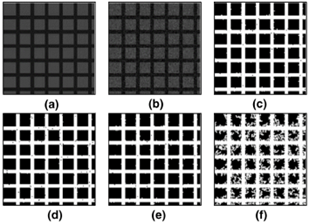
\includegraphics[width=0.5\textwidth]{figures/人工图像测试.png}
    \caption{(a) 原始图像; (b) 带高斯噪声的原始图像; (c) 当α=αmax的最佳分割区域;最佳区域: (d) 依据w1, w2, w3; (e) 依据V 和 InvDGL; (f) 依据 S.}
    \label{fig:人工图像测试}
\end{figure}

\begin{figure}[htbp]
    \centering
    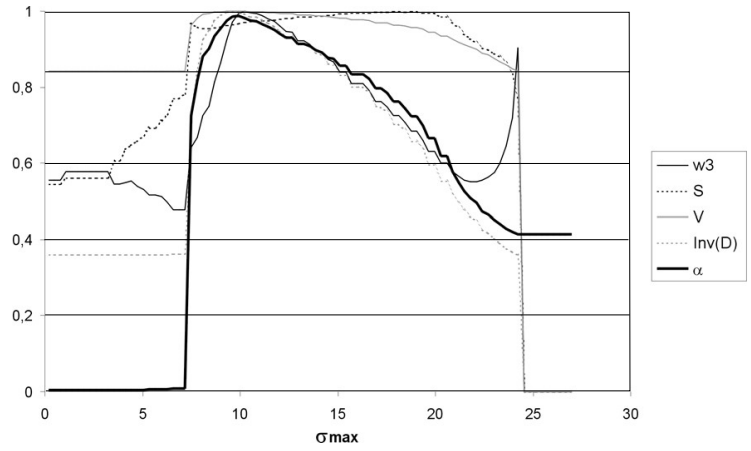
\includegraphics[width=0.5\textwidth]{figures/评估函数.png}
    \caption{系数α和由w1,w2,w3,S,V,InvDGL计算的归一化评估函数与σmax的关系}
    \label{fig:评估函数}
\end{figure}

\clearpage
\section{基于图序列生成标定结果}\label{sec:4}

在上述流程中,我们对视频数据中的每一帧生成了一张对应的蒙版。该蒙版记录了钡餐区域的本底值数据。现在我们来到了最后一部分,即基于这些本底值数据得到最终的钡餐区域和浓度标定结果。

\subsection{定义}\label{sec:4_1}
\begin{itemize}
    \item 我们将一组(经过预处理后的)医学视频数据记为 $D$。其中第 $k$ 帧所代表的二维灰度图像为 $D[k]$。该图像中像素 $[x, y]$ 处的灰度值为 $D[k, x, y]$。
    \item 我们将通过 $D[k]$ 所求得的视频第 $k$ 帧对应的钡餐区域及其本底值记为 $T[k]$。对于 $T[k]$ 中的像素 $[x, y]$,记 $T[k, x, y]=t$。若 $t=0$,代表该像素在该帧中非钡餐区域;反之,代表该像素在该帧属于钡餐区域,且算法认为该像素点在成为钡餐区域之前,其所对应的人体器官或组织的像素值为t。在最终逐帧逐像素标记钡餐浓度时,应根据此本底值做出修正。
    \item 对于数组 $T$,维护一个与之一一对应的布尔数组 $F$。若 $F[i]$ 为真,代表尝试使用 $T[i]$ 进行扩张,反之不使用。
    \item 我们将最终的钡餐区域及浓度标定结果数据记为 $R$。对于第 $k$ 帧中的像素 $[x, y]$,记 $R[k, x, y]=r$。若 $r=0$,代表该像素在该帧中非钡餐区域;反之,代表该像素在该帧中属于钡餐区域,且其相对浓度为 $r$。$r$ 的取值范围为 $[0, 255]$,数值越大代表其相对浓度越高。
\end{itemize}

\subsection{方法描述}

事实上,在上述流程中,每一帧求得的钡餐本底值蒙版不一定能完整地标注出钡餐区域。由于该蒙版是通过绝对差图像处理得到的,因此当且仅当某一帧中整个钡餐区域的边界相较上一帧在各个方向都有的运动时,蒙版中的钡餐区域才具有较高的准确度。在实际数据中,受试者将钡餐含在口中不咀嚼时,钡餐的运动可能较为平缓;而受试者在吞咽钡餐时,钡餐沿着喉管运动,其方向沿着呈现强烈的指向性。在这些情景下,绝对差图像中无法表现出完整的轮廓,进而导致钡餐区域标注不准确。在\cref{fig:4_示意图} 中,我们用一组简化的图像说明该情况。

\begin{figure}[!htp]
    \centering
    \begin{subfigure}{\textwidth}
        \centering
        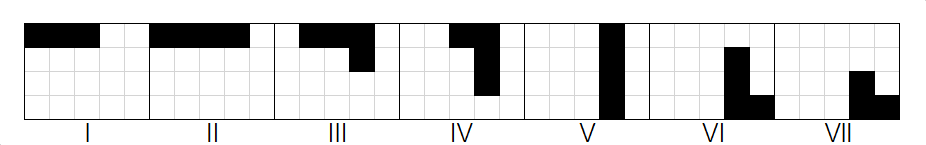
\includegraphics[width=0.8\textwidth]{figures/4_示例_1.png}
        \caption{原始数据}
    \end{subfigure}
    \begin{subfigure}{\textwidth}
        \centering
        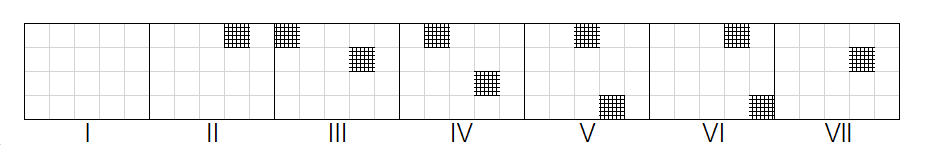
\includegraphics[width=0.8\textwidth]{figures/4_示例_2.png}
        \caption{运动区域}
    \end{subfigure}
    \begin{subfigure}{\textwidth}
        \centering
        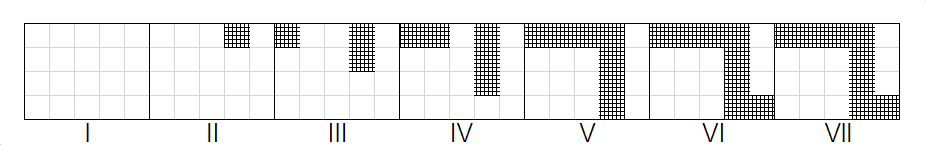
\includegraphics[width=0.8\textwidth]{figures/4_示例_3.png}
        \caption{运动区域叠加}
    \end{subfigure}
    \begin{subfigure}{\textwidth}
        \centering
        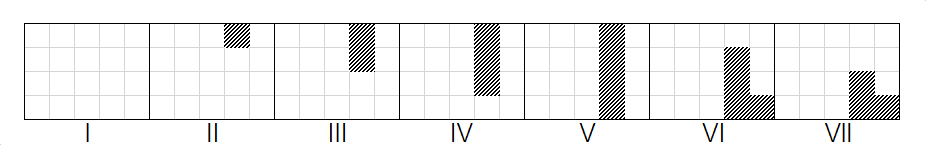
\includegraphics[width=0.8\textwidth]{figures/4_示例_4.png}
        \caption{运动区域叠加后与原始数据求交}
    \end{subfigure}
    \caption{简化示意图}
    \label{fig:4_示意图}
\end{figure}

在\cref{fig:4_示意图}(a) 中,我们展示了一组钡餐的运动过程,共7帧。每一帧中的黑色的部分代表钡餐。在图中,钡餐首先被拉伸,随后向下移动至底部拐弯,最后收缩。\cref{fig:4_示意图}(b) 展示了原始数据的绝对差图像,其中方格部分代表该帧与前一帧不同之处,即钡餐的运动部分。观察可知,在该样例下,通过绝对差图像最终得到的蒙版无法与实际钡餐区域准确对应。

为解决此问题,需充分利用连续时间段内所有图像的信息,而非仅关注相邻帧间的差异。我们可以注意到以下结论:除第一帧中钡餐所在的区域,若某坐标在某帧属于钡餐区域,则该坐标必然在此帧或其前驱帧中从非钡餐区域转变为钡餐区域。如果我们将\cref{fig:4_示意图}(b) 中的每帧与其所有前驱帧叠加,可得到\cref{fig:4_示意图}(c),每帧图像表示截至当前帧,所发现的所有当前或曾经属于钡餐的区域。\cref{fig:4_示意图}(d) 展示了将 (c) 图与 (a) 图取交集的结果。如此一来,除初始几帧外,(d) 中的后续帧与原始数据吻合。这说明(c) 中(除初始几帧外)的图像可以在将原始数据的大部分区域过滤的同时,保留足够多的感兴趣区域,不遗漏。

在实际数据中,两个帧本底值蒙版之间的操作并不能单纯用“叠加”来概括。因为蒙版并非一个二值图,而是灰度图。我们需要设计相应的方法来处理。此外,在实际操作过程中,我们并不能直接将每一帧与其所有前驱帧叠加,再执行所谓的“求交”操作。因为钡餐区域正是需要我们寻找的目标,而非预先已知的数据。即意味着,我们需要构建某种方法以判断和记录每个帧蒙版的有效性,需要决定每一帧使用哪些前驱帧进行扩展,需要判断何时终止扩展以达到最佳效果。何况,在处理每一帧时,叠加所有前驱帧结果本身便会导致性能问题。

\subsection{操作流程}

在本研究中,对于本底值蒙版数组 $T$,我们维护一个与之一一对应的布尔数组 $F$。若 $F[i]$ 为真,代表尝试使用 $T[i]$ 进行扩张,反之不使用。我们将当前最前驱的有效帧记为 $e$,即:$F[0]=F[1]=...=F[e-1]=\text{False}, F[e]=\text{True}$。

对于第 $i$ 帧,求取 $R[i]$ 的具体步骤如下:
\begin{itemize}
    \item 将 $T[i]$ 的数据拷贝给 $R[i]$。
    \item 对 $i-1$ 到 $e$ 中的每一帧 $k$:
    \subitem 若 $F[k]$ 为真,则使用 $T[k]$ 对 $R[i]$ 进行\textit{扩张}。
    \subitem 若 $T[k]$ 未能更新 $R[i]$ 中的任何一个像素点,则 $F[k]$ 置为假,后续不再考虑第 $k$ 帧。
    \item 更新 $e$ 的值。
    \item $R[i] = R[i] - D[i]$
\end{itemize}

其中,扩张过程遵循以下约定:若第 $k$ 帧中的坐标 $[x, y]$ 的本底值 $T[k, x, y]$ 大于该坐标在第 $i$ 帧的数据值 $D[i, x, y]$,且同时大于 $R[i, x, y]$,则将 $T[k, x, y]$ 赋值给 $R[i, x, y]$。

扩张过程的伪语言描述如下:
\begin{algorithm}
    \caption{扩张过程}\label{algo:expansion}
    \begin{algorithmic}[1]
        \Require 当前帧图像 $d$, 当前帧标定结果 $r$, 待使用的蒙版 $t$
        \Ensure 更新后的帧标定结果 $r$, $r$ 中被蒙版 $t$ 更新的像素数量 $p$
        \Function{ExpandArea}{$d, r, t$}
            \State $x, y \gets d.shape$ % x, y = d.shape
            \State $p \gets 0$ % p = 0
            \For{$i \in \{0, \cdots, x-1\}$} % for i in range(x):
                \For{$j \in \{0, \cdots, y-1\}$} % for j in range(y):
                    \If{$t[i][j] \geq d[i][j]$} % if t[i][j] >= d[i][j]:
                        \If{$t[i][j] > r[i][j]$} % if t[i][j] > r[i][j]:
                            \State $p \gets p + 1$ % p += 1
                            \State $r[i][j] \gets t[i][j]$ % r[i][j] = t[i][j]
                        \EndIf
                    \EndIf
                \EndFor
            \EndFor
            \State \Return $p$ % return p
        \EndFunction
    \end{algorithmic}
\end{algorithm}

\subsection{结果}

由于原始采集仪器数据及环境数据暂缺,无法确定钡餐的绝对浓度,因此以下结果中,浓度标定均采用相对浓度。\cref{fig:4_结果} 展示了两组经过上述操作后得到的钡餐区域和浓度标注。这两组数据中,钡餐分别位于受试者的口部和喉部。每组数据中,从左到右分别为:原始数据帧,由相邻帧得到的钡餐区域及蒙版,使用本章方法扩展得到的钡餐区域及浓度标定。
其中,黑色部分代表非钡餐区域;非黑色部分其亮度越高,代表其相对浓度越高。
\clearpage
\begin{figure}[!htp]
    \centering
    \begin{subfigure}{\textwidth}
        \centering
        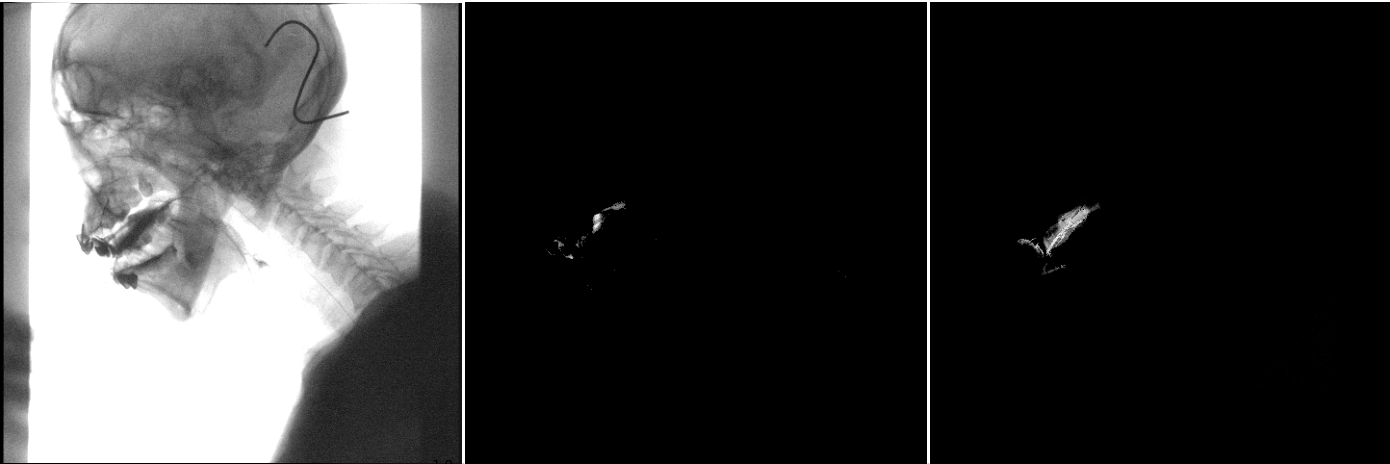
\includegraphics[width=0.9\textwidth]{figures/421.png}
        \caption{口部}
    \end{subfigure}
    
    \begin{subfigure}{\textwidth}
        \centering
        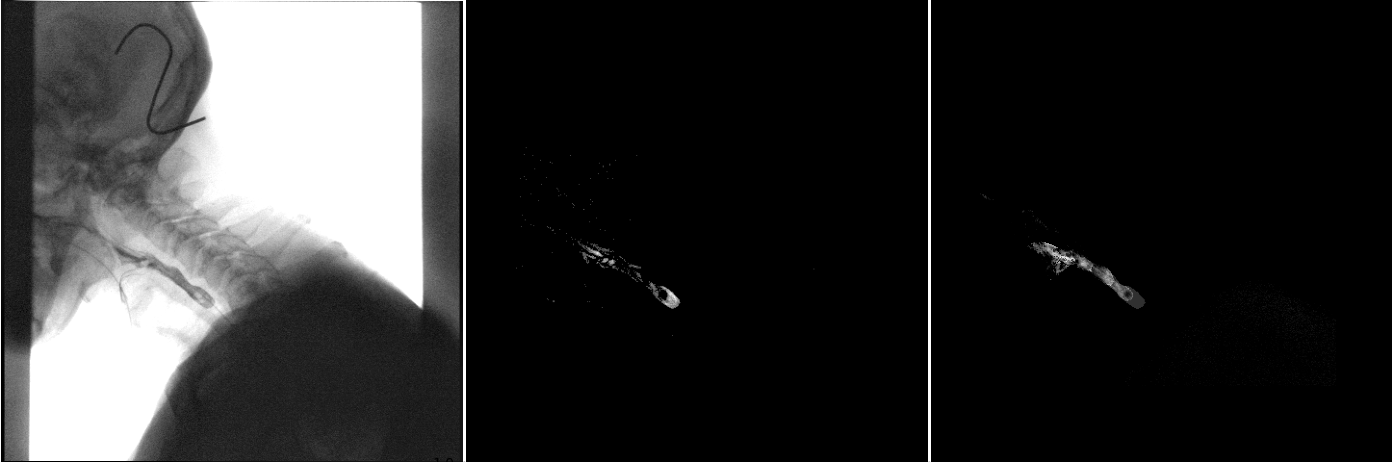
\includegraphics[width=0.9\textwidth]{figures/422.png}
        \caption{喉部}
    \end{subfigure}
    \caption{钡餐区域和相对浓度标注}
    \label{fig:4_结果}
\end{figure}

\subsection{本章小结}

本章中,我们提出一种拓展逐帧操作成果的算法。针对每一帧图像,以上述获得的蒙版作为基础,借助前驱帧所得蒙版进行扩张操作;在此过程中,不断维护各蒙版的有效性,以提高处理速度。最终,我们得到每一帧中的钡餐区域及相对浓度标定。
\clearpage
\section{实验结果分析}\label{sec:-2}

本研究获取了合作医院的人类食道的医学造影数据,涉及 4 名患者共计 28 个影像数据。所得数据为患者头颈部侧位DR图像,采用连续采集方式生成视频。图像分辨率为 $480 \times 480$,每个视频的帧数介于 100 至 500 帧之间。

本实验采用 Windows11 操作系统,搭载 AMD R7-3700x @ \SI{3.6}{\giga\hertz} CPU 的个人电脑进行实验评估。代码使用 Python 语言编写,完成了完整的可运行 demo。使用本文方法,处理 $480 \times 480$,400帧规模的DICOM医学影像数据并输出结果,时间消耗约 20 秒。demo 未经多核优化,未使用 GPU,在运行效率上有较大提升空间。

本研究的最终输出结果为视频格式,视频的每一帧图像包括2个子图:原始数据帧图像,以钡餐范围及浓度标定图像。后者以R通道输出,同时取原始图像的20\%亮度作正片叠底。\cref{fig:5_结果1} 和\cref{fig:5_结果2} 是部分数据的输出结果中的截图。
\begin{figure}[!htp]
    \centering
    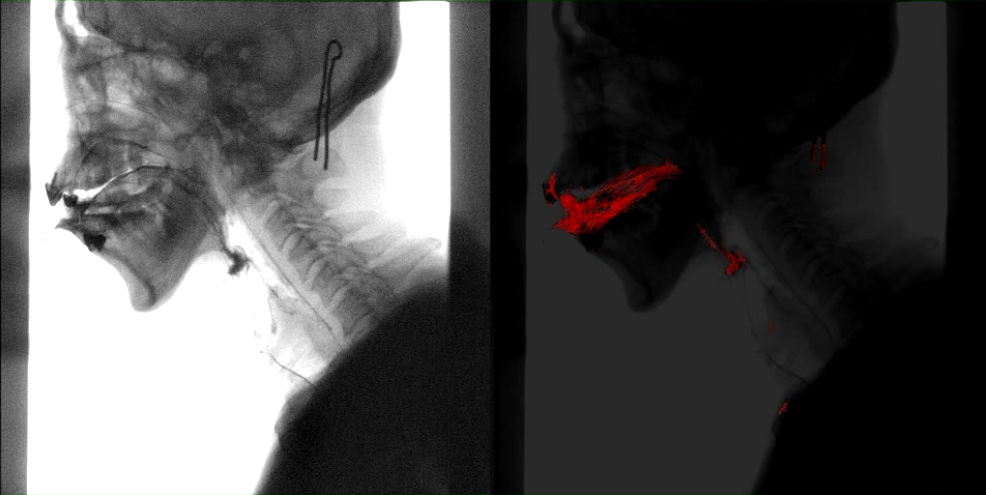
\includegraphics[width=0.8\textwidth]{figures/511.png}
    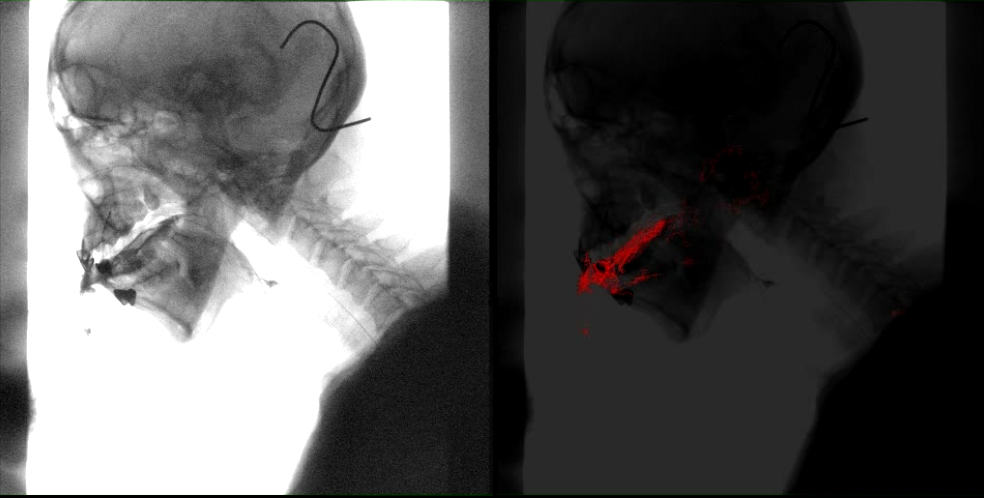
\includegraphics[width=0.8\textwidth]{figures/513.png}
    \caption{钡餐标定结果-口部}
    \label{fig:5_结果1}
\end{figure}

\begin{figure}[!htp]
    \centering
    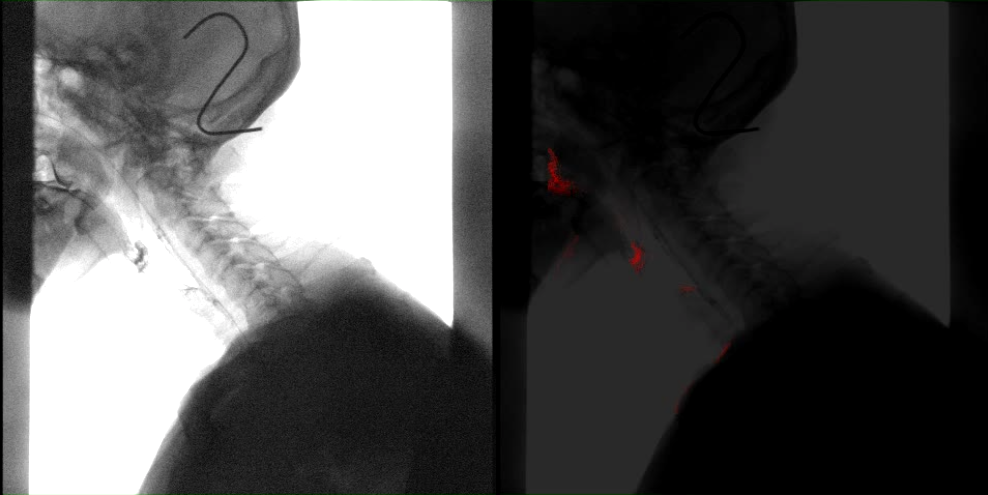
\includegraphics[width=0.8\textwidth]{figures/512.png}
    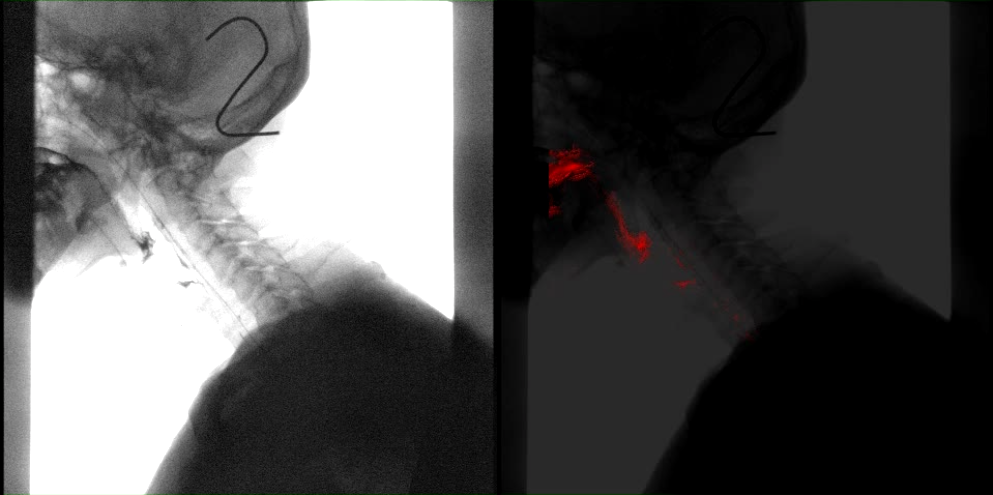
\includegraphics[width=0.8\textwidth]{figures/514.png}
    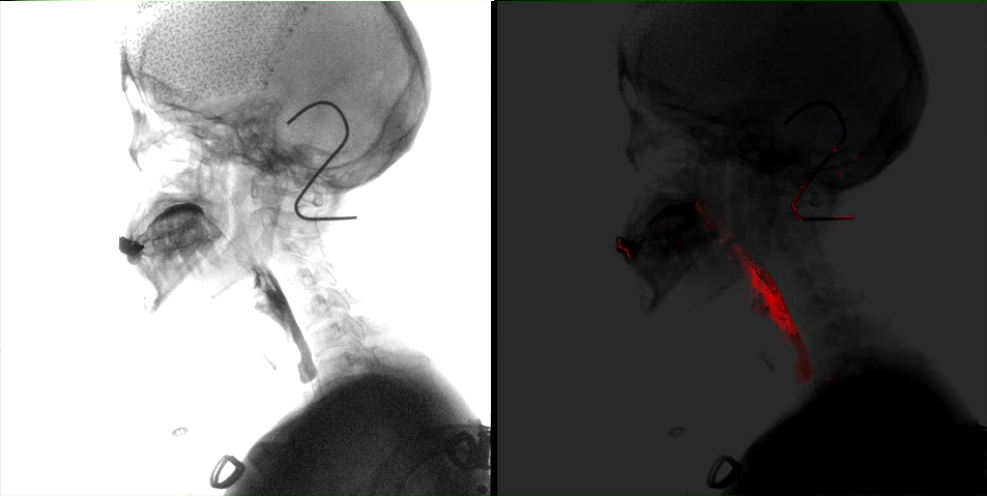
\includegraphics[width=0.8\textwidth]{figures/515.png}
    \caption{钡餐标定结果-喉部}
    \label{fig:5_结果2}
\end{figure}

针对DR图像的分割、标定或三维重建算法的评估,通常会采用相应的MR图像或CT图像作为基准进行对比。然而,本研究涉及的视频数据无法通过这些方法获得。在缺乏更高级设备参考的情况下,通常需要医学专家手动标注以获取标准图像集。然而遗憾的是,本研究仅获得了原始数据,并未获得标准图像集,因此无法通过准确率、精确率、召回率、$F_1$分数或ROC曲线等指标来评估结果。此外,本课题研究内容具备创新性,目前尚未见相关研究或算法模型,暂缺乏与其他方法的结果对比分析。综上,本项目在综合考虑正负样本指标的基础上,采纳了一套以人工观察为主要依据的评价指标。

首先,我们对钡餐在受试者体内各器官的分布情况进行了统计。我们将数据按钡餐在口部出现和在喉部出现分为两类。特别的,若在某组数据中钡餐先后出现在了口部和喉部,我们将该数据的两个副本分别放入两类中。统计表明,钡餐在 82.1\% 的数据中出现在口部,在 60.7\% 的数据中出现在喉部。

接下来,我们对每组数据的处理结果做出评价。评价分为以下类别:
\begin{itemize}
    \item 漏标:存在未被标记的钡餐区域(假阴)。
    \item 多标:不存在漏标,但存在将非钡餐区域标记为钡餐区域(假阳)。
    \item 明显损失:不存在错标,但对钡餐区域的标记存在明显损失,不够完整。
    \item 明显溢出:不存在错标和明显损失,但对钡餐区域的标记存在明显溢出。
    \item 准确:不存在任何以上问题。
\end{itemize}

依照该准则,我们对实验结果进行了评估和统计,详见\cref{tab:5_result}。
\begin{table}[!htbp]
    \centering
    \begin{threeparttable}[b]
        \caption{观察结果}
        \label{tab:5_result}
        \begin{tabular}{@{}lrrrrrrrrrrrrrr@{}}
            \toprule
                & \multicolumn{2}{c}{\textbf{原始数据}} & \multicolumn{2}{c}{\textbf{多标}} & \multicolumn{2}{c}{\textbf{漏标}} & \multicolumn{2}{c}{\textbf{明显溢出}} & \multicolumn{2}{c}{\textbf{明显损失}} & \multicolumn{2}{c}{\textbf{准确}}\\
            \cmidrule(lr){2-3} \cmidrule(lr){4-5} \cmidrule(lr){6-7} \cmidrule(lr){8-9} \cmidrule(lr){10-11} \cmidrule(lr){12-13} \cmidrule(lr){14-15}
                \textbf{器官} & \textbf{数量} & \textbf{占比} & \textbf{数量} & \textbf{占比} & \textbf{数量} & \textbf{占比} & \textbf{数量} & \textbf{占比} & \textbf{数量} & \textbf{占比} & \textbf{数量} & \textbf{占比} \\
            \midrule
                口部            & 25      & 100\% & 7      & 28\% & 1      & 4\% & 8      & 32\% & 1      & 4\% & 8      & 32\%  \\
                喉部            & 17      & 100\% & 0      &  0\% & 0      & 0\% & 8      & 47\% & 1      & 6\% & 8      & 47\%  \\
            \bottomrule
        \end{tabular}
    \end{threeparttable}
\end{table}

分析表中数据可得,本研究的方法应用在喉部数据时尚可,应用于口部数据时欠佳。所有数据的标定结果中,出现漏标和明显损失的占比较少。喉部数据未见错标。错误主要集中在对钡餐区域的标记范围明显溢出,以及口部数据中对非钡餐区域出现了误标。

对于多标错误的数据进行分析发现,有时本文方法会将受试者的后脑勺,患者的衣领,以及护士的袖口等非钡餐区域标记为钡餐区域。这类错误可以通过各种技巧在后处理阶段排除。在实际应用中,这类错误对诊断的影响较小。我们的主要关注点仍然是算法对钡餐在受试者的口、咽、喉部的标定准确度。针对大量数据的标注结果标记范围明显溢出的问题,我们总结了以下原因和改进方案:
\begin{enumerate}
    \item 在行光流法配准时,我们主要以头部轮廓作为配准依据。然而我们观察到,在俯仰动作较大的数据中,头部轮廓的运动矢量和喉管的运动矢量差异巨大,导致配准后的图像中,喉管的位置和实际并不匹配,最终导致标注结果差,在极端情况下,结果甚至不如不进行配准。我们认为一个可行的改进方案为:使用卷积神经网络准确分割出喉管,直接对喉管进行配准。
    \item 我们发现在以下情景中,标注结果会出现明显溢出:护士通过针筒将钡餐注入受试者口腔后,立即用手掌拖住受试者下颌,向上移动下颌来使嘴部闭合,防止钡餐直接流出。此时,嘴部的运动矢量明显大于图像中的其它部位,导致算法将几乎整个嘴部均标记为钡餐区域。我们认为一个可行的改进方案为:对图像进行光流分析时,动态地将图像中“活跃”(即:运动矢量值明显高于整个图像的平均值)的局部提取出来。对该局部单独进行窗宽窗位调整和钡餐区域标定分析。
\end{enumerate}

除此之外,由于本研究主要基于帧间运动信息计算得到最终结果,因此每组影像数据的最初几帧的标注结果通常不够理想。在实验中,钡餐由护士通过针筒注入受试者口腔,应在注射前即开始DR图像的记录。但在实际影像数据中,部分记录始于钡餐已进入受试者口腔后。针对此类数据的标注结果通常出现明显损失甚至漏标。我们认为一个可行的改进方案为:为用户提供一套操作界面,允许研究人员在影像数据的首帧中手动勾画钡餐区域轮廓。在此过程中,可辅以区域生长算法\cite{REVOLMULLER2002137}帮助用户进行标注,根据用户所选坐标点生长出一片标记区域,将轮廓勾画操作简化为多次点选与微调。    

在浓度的标定方面,由于原始采集仪器数据及环境数据暂缺,无法确定钡餐的绝对浓度。在获取原始采集仪器数据及环境数据后,可以根据相关公式计算出绝对浓度值标定。同时还需获取专家的标定结果,方可得到进一步的评价指标,包括:钡餐范围与实际范围重合度、钡餐标定浓度与实际浓度平均方差等。

\clearpage
\section{总结与展望}\label{sec:-1}

\subsection{总结}

本课题对人类食道医学造影视频进行分析,标注出不同浓度钡餐在食道内的分布区域。本课题所涉及的数据样本规模较小,目标形态差异较大,且对标注精度要求高。经查阅,目前尚缺相关的研究成果与算法模型,研究内容具有创新性,难度较大。本课题运用多种医学图像处理方法,以及计算机视觉和图形学领域的方法,结合自己的优化,完成了该工程实践与挑战。

本课题处理的数据为头颈部侧位X线检查所得的DR图像经短时连续采集而得到的视频。本课题输出的数据为与输入数据同规格的视频,其中每一帧为钡餐范围及浓度标定图像。在研究中,我们对每组输入数据依次进行以下处理:
\begin{enumerate}
    \item 使用自动窗宽窗位算法,标准化输入数据。
    \item 使用光流法对视频数据进行配准,尽可能抵消受试者的头部整体运动,以使后续对钡餐运动矢量的提取更准确。
    \item 对视频中的每一对相邻帧图像进行处理,获取一组代表本底值的像素点。具体步骤如下:
    \subitem 对相邻帧图像求差,得到差值灰度图。
    \subitem 使用双边滤波对灰度图降噪。
    \subitem 对降噪后图像行二值化。
    \subitem 使用膨胀腐蚀等形态学操作对二值图进一步降噪。
    \subitem 使用铃木算法从二值图中获取轮廓。
    \subitem 使用格林公式计算各轮廓所包围的面积,快速过滤噪点小轮廓,保留感兴趣的大轮廓。
    \subitem 对每个过滤后留下的轮廓,使用泛洪法填充算法获取轮廓所包围的像素点的集合。
    \subitem 基于相邻两帧的信息,赋予集合中的每个像素点本底值。
    \item 为进一步利用视频所包含的运动信息,对于每个新求得的本底值蒙版,使用之前得到的蒙版进行扩张操作。
    \item 将扩张后的蒙版与当前帧数据进行运算,得到每一帧的钡餐区域和相对浓度标定。
    \item 将每一帧标定结果组合成连续帧,得到输入数据同规格的视频并输出。
\end{enumerate}

由于缺乏标准集,我们自定义了一套以人工观察为主要依据的评价指标。分析结果得到以下结论:本研究方法对喉部的标定结果尚可,对口部的标定。错误主要集中在对钡餐区域的标记范围明显溢出,以及口部数据中对非钡餐区域出现了误标。我们总结问题并提出改进方案,但由于个人精力和能力等原因,在本科阶段的研究暂止步于此。

\subsection{展望}

当前的标定结果的准确度尚不足以进入实际使用。在接下来的研究中,我们首先尝试实现\cref{sec:-2} 中对实验结果分析后所提出的各个改进方案以提高钡餐标定准确度。我们需获取更多的数据集,以及经医学专家手动标注的标准集。

若项目进展顺利,后续我们还将面临更艰难的挑战。我们需通过不同粘稠度的钡餐在食道内流动形成的封闭几何区域来确定会厌软骨的位置,并追踪其在吞咽过程中连续的运动轨迹。接下来,我们尝试标定钡餐被会厌软骨罩住的容积,以及侧漏发生时气管所处的部位与会厌软骨相对位置。随后,我们将基于流动参数和运动形态变化,结合动力学模型,实现三维模型的重建。最后,我们需对不同粘稠度的钡餐的运动过程进行三维仿真,从而为医师提供可视化的诊断治疗辅助手段。
\clearpage

\phantomsection % 添加占位符章节
\addcontentsline{toc}{section}{参考文献}
\printbibliography[heading=bibliography,title=参考文献]

\clearpage
\section*{谢\ 辞}
\addcontentsline{toc}{section}{谢辞}

这项工作属于法国国家科学研究中心(CNRS)的PRC-GdR ISIS和GDR 2237研究小组的科学课题范围。作者非常感谢法国里昂CPE核磁共振实验室的Pr. André Briguet先生提供的三维磁共振图像。他们还感谢Olivier Beuf博士对MR图像的采集。

\end{document}
